% Tags: 4321102, parallel, shift, parallel-in, working, register
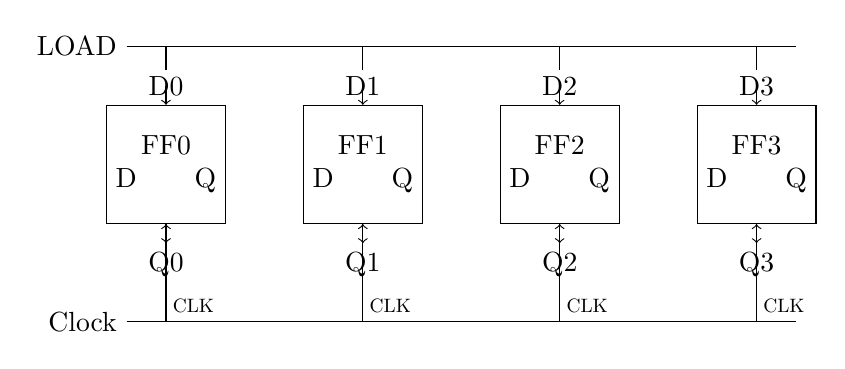
\begin{tikzpicture}[
    node distance=2cm,
    auto,
    block/.style={rectangle, draw, minimum width=1.5cm, minimum height=1.5cm, align=center}
]
    \foreach \i in {0,1,2,3} {
        \node[block] (FF\i) at (\i*2.5, 0) {FF\i\\D \hspace{0.5cm} Q};
        \node[above] at (FF\i.north) {D\i};
        \draw[->] (\i*2.5, 1) -- (FF\i.north);
        \draw[->] (FF\i.south) -- (\i*2.5, -1) node[below] {Q\i};
        \draw[->] (\i*2.5, -2) -- (\i*2.5, -1.8) node[right, scale=0.7] {CLK} -- (FF\i.south); % Visual clock
    }
    
    % Clock Line
    \draw (-0.5, -2) node[left] {Clock} -- (8, -2);
    
    % Load control (simplified as LOAD signal usually enables clock or D inputs)
    \draw (-0.5, 1.5) node[left] {LOAD} -- (8, 1.5);
    \foreach \i in {0,1,2,3} {
        \draw (\i*2.5, 1.5) -- (\i*2.5, 1.2);
    }

\end{tikzpicture}
